


\textbf{Прошедшая волна}.
Обозначим через $R$ коэффицент отражение света от границы раздела пластинки с воздухом. При отсутсвии поглощения $(1-R)$ проходит через границу, если среды по обе стороны одинаковы, то и $R$ будут одинаковы. Пусть свет монохроматичен
Пусть интенсивность света $I_0$, тогда интенсивности прошедших пучков будут
\begin{equation*}
    I_{1'} = (1-R)^2, \hspace{5 mm} 
    I_{2'} = R^2(1-R)^2 I_0, \hspace{5 mm} 
    I_{3'} = R^4 (1-R)^2 I_0, \hspace{5 mm}  \ldots
\end{equation*}
а соответсвеющие вещественные амплитуды
\begin{equation*}
    a_{1'} = (1-R) a_0, \hspace{5 mm} 
    a_{2'} = R(1-R) a_0, \hspace{5 mm} 
    a_{3'} = R^2(1-R) a_0, \ldots .
\end{equation*}
Амплитула прошедшей волны представится убывающей геометрической прогрессией
\begin{equation*}
    \sub{a}{d} = a_0 (1-R)\left[1 + R e^{-i \Phi} + R^2 e^{-2i \Phi} + \ldots\right],
    \hspace{5 mm} 
    \Phi = k \Delta = \frac{4 \pi}{\lambda} n d \cos \psi,
    \hspace{0.5cm} \Rightarrow \hspace{0.5cm}
    \sub{a}{d} = \frac{1-R}{1-R e^{-i\Phi}} a_0.
\end{equation*}
где $\Phi$ -- разность фаз между соседними пучками.  Интенсивность прошедшей волны
\begin{equation*}
    \sub{I}{d} = \frac{(1-R)^2}{|1-R e^{-i \Phi}|^2} a_0^2 = \frac{(1-R)^2}{(1-R)^2 + 4 R \sin^2 (\Phi/2)} I_0,
\end{equation*}
что позволяет сделать некоторые выводы. 



\textbf{Отраженная волна}. Аналогичный расчёт приведет к
\begin{align*}
    &I_1 = R I_0, 
    &I_2 = R(1-R)^2 I_0, 
    &&I_3 = R^3 (1-R)^2 I_0, 
    &&\ldots, \\ 
    &a_1 = \sqrt{R} a_0, 
    &a_2 = - \sqrt{R} (1-R) a_0, 
    &&a_3 = - \sqrt{R} R (1-R) a_0, 
    &&\ldots,
\end{align*}
где знак в $a$ -- следставие появления $\lambda/2$. Резуьтирующая амплитуда будет иметь вид
\begin{equation*}
    a_r = \sqrt{R} a_0 - \sqrt{R} (1-R) a_0 e^{-i \Phi} \left[
        1 + R e^{- i \Phi} + R^2 e^{-2i \Phi} + \ldots
    \right],
    \hspace{0.5cm} \Rightarrow \hspace{0.5cm}
    I_r = \frac{4 R \sin^2 (\Phi/2)}{(1-R)^2 + 4 R \sin^2(\Phi/2)} I_0, 
\end{equation*}
где всё также $\Phi = k \Delta = \frac{4 \pi}{\lambda} n d \cos \psi$.


При $R \ll 1$ увидим случай двулучевой интерференции, при $R \approx 1$ уже интереснее (рис. \ref{fig:piks}). 
\begin{figure}[ht]
    \centering
    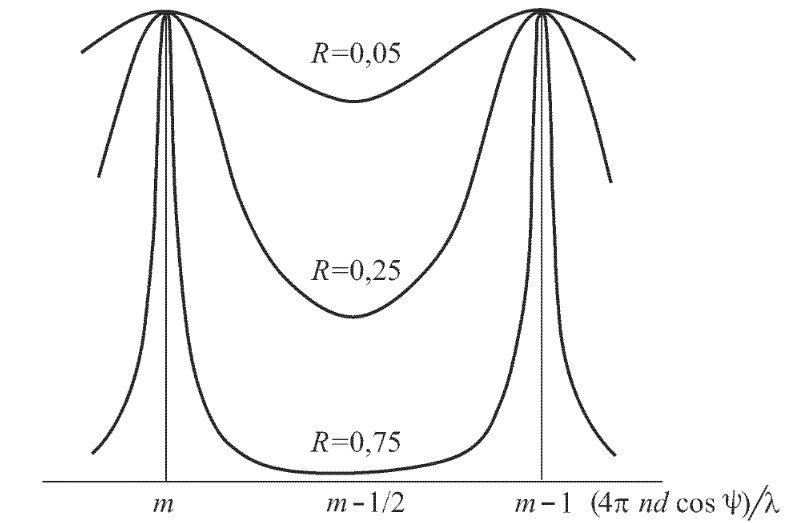
\includegraphics[width=0.3\textwidth]{figures/36_1.png}
    \caption{Пики для пластинки}
    \label{fig:piks}
\end{figure}
В окрестности максимума $m$-го порядка $\Phi = \pi m + \varphi$, тогда ввиду малости $\varphi$ можем написать
\begin{equation*}
    \sub{I}{d} = \frac{I_{\text{max}}}{1 + R \varphi^2/(1-R^2)},
    \hspace{0.5cm}
    \frac{R \varphi^2}{(1-R)^2} = 1 \text{ при } \sub{I}{d}= \frc{1}{2} \sub{I}{max},
    \hspace{0.5cm} \Rightarrow \hspace{0.5cm}
    \Delta \Phi = 2 \varphi = 2 \frac{1-R}{\sqrt{R}}.
\end{equation*}

